% Documentation for draw block - Jonathan Ely
\documentclass[11pt,a4paper]{article}
\usepackage{graphicx}
\title{Draw Block Documentation}
\author{Jonathan Ely}

\begin{document}
\maketitle
\section{Introduction}
The Draw Block is responsible for taking input commands from the host processor,
decoding them and passing the pixel operations to the RAM Control Block.
It is comprised of three VHDL entities: 
\emph{draw\_block}, \emph{draw\_any\_octant} and \emph{draw\_octant}.

\section{draw\_block}
This is the top entity for the draw block and supports interfaces for
the host and the RCB. The main job of this block is to decode the host commands
and provide pixel operations to the RCB. It is implemented as a 3 state FSM,
as shown in fig 1.

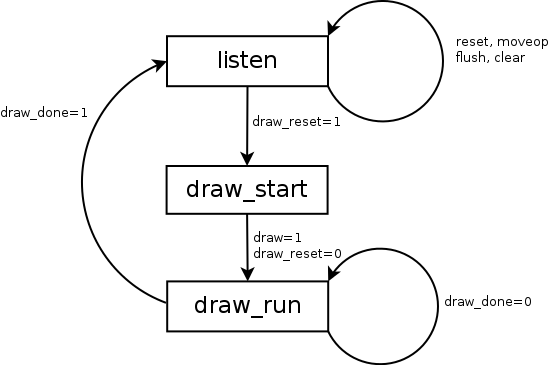
\includegraphics[scale=0.5]{drawfsm.png}

In order to calculate the draw operations, the draw block creates a wrapper for 
the \emph{draw\_any\_octant} entity from exercise 4. 

\subsection{SIGS: PROCESS}
This combinational process decodes the \emph{hdb} signal from the host processor
into its more useful component parts: \emph{xin}, \emph{yin}, \emph{pen} and \emph{op}.

\subsection{OCT: PROCESS}
This process compares the x and y input positions to the pen position to work
out which octant we want to draw in. It is used by the \emph{draw\_any\_octant}
entity.

\subsection{STATECOMB: PROCESS}
STATECOMB manages the state of the FSM. It also implements the Move Pen,
Clear and Flush operations as they only take 1 cycle. For the draw command, it sets up the \emph{draw\_any\_octant module} with the start position
(by holding the \emph{draw\_reset} signal high) and passes to the
\emph{draw\_start} state.

\subsection{FSM: PROCESS}
This clocked process increments the state with the \emph{nstate} signal
on the rising edge of the clock. There are two cases when this does not happen:
when \emph{delaycmd} is high or when \emph{reset} is high. 
The \emph{delaycmd} signal is set by the RCB and stops state progression.
The \emph{reset} signal returns the state to \emph{listen}. 

\section{draw\_any\_octant - Exercise 4}
This the \emph{draw\_any\_octant} entity from exercise 4. It's job is to
translate the input/output to \emph{draw\_octant} so that it can draw in
any of the 8 octants: NNE, ENE, ESE, SSE, SSW, WSW, WNW and NNW.

It has been modified slightly to allow halting whilst the RCB is busy.
This is achieved by stopping the clocked process whilst \emph{delay} is high.

\section{draw\_octant - Exercise 1}
This is the \emph{draw\_octant} entity from exercise 1.
It has been modified slightly to allow halting whilst the RCB is busy.
This is achieved by stopping the clocked process whilst \emph{delay} is high.


\end{document}

